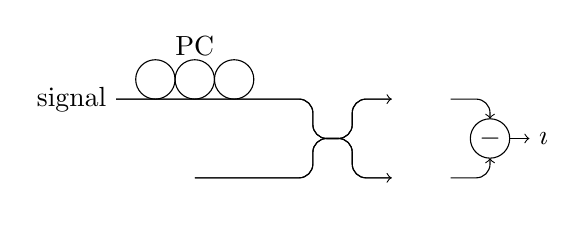
\begin{tikzpicture}
    \draw[rounded corners=5pt] (0.5,0)node[left]{signal} --++ (2.5,0) --++ (0,-0.5) --++ (0.5,0) --++ (0,0.5) --++ (0.5,0);
    \draw[rounded corners=5pt,->] (0.5,0) --++ (2.5,0) --++ (0,-0.5) --++ (0.5,0) --++ (0,0.5) --++ (0.5,0);
    \draw (1,0.25) circle (0.25);
    \draw (1.5,0.25) circle (0.25) node[above = 5pt]{PC};
    \draw (2.0,0.25) circle (0.25);
    
    \draw[rounded corners=5pt] (1.5,-1) --++ (1.5,0) --++ (0,+0.5) --++ (0.5,0) --++ (0,-0.5) --++ (0.5,0);
    \draw[rounded corners=5pt, ->] (1.5,-1) --++ (1.5,0) --++ (0,+0.5) --++ (0.5,0) --++ (0,-0.5) --++ (0.5,0);
    
    \draw[rounded corners=5pt,->] (4.75,0) --++ (0.5,0) --++ (0,-0.25);
    \draw[rounded corners=5pt,->] (4.75,-1) --++ (0.5,0) --++ (0,+0.25);

    \draw (5.25,-0.5) circle (0.25)node{$\bm{-}$};
    \draw[->] (5.5,-0.5) --++ (0.25,0) node[right]{$\imath$};
    \laserSize{2.25}{-2}{black}{0.5}{LO}
    \PD{8.75}{-2}{black}{0.5}
    \PD{8.75}{0}{black}{0.5}

    \draw[white] (0,-1.5) --++ (2,0);
\end{tikzpicture}
